 \documentclass{article}
\usepackage[utf8]{inputenc}
\usepackage[a4paper, total={7in, 10in}]{geometry}
\usepackage{braket}
\usepackage{xcolor}
\usepackage{amsmath}
\usepackage{amssymb}
\usepackage{amsfonts}
\usepackage{graphicx}
\usepackage{svg}
\usepackage{float}
\usepackage{tikz}
\usepackage[ruled,vlined]{algorithm2e}
\usepackage{multicol}
\usepackage[backend=biber,style=alphabetic,sorting=ynt]{biblatex}
\usepackage{xcolor}
%\addbibresource{sample.bib} %Import the bibliography file

\newcommand{\commentt}[1]{\textcolor{blue}{ \textbf{[COMMENT]} #1}}
\newcommand{\ctt}[1]{\commentt{#1}}
\newcommand{\prb}[1]{ \mathbf{Pr} \left[ {#1} \right]}
\newcommand{\onotation}[1]{\(\mathcal{O} \left( {#1}  \right) \)}
\newcommand{\ona}[1]{\onotation{#1}}
\newcommand{\PSI}{{\ket{\psi}}}
\newcommand{\LESn}{\ket{\psi_n}}
\newcommand{\LESa}{\ket{\phi_n}}
\newcommand{\LESs}{\frac{1}{\sqrt{n}}\sum_{i}{\ket{\left(0^{i}10^{n-i}\right)^{n}}}}
\newcommand{\Hn}{\mathcal{H}_{n}}
\newcommand{\Ep}{\frac{1}{\sqrt{2^n}}\sum^{2^n}_{x}{ \ket{xx}}}
\newcommand{\HON}{\ket{\psi_{\text{honest}}}}
\newcommand{\Lemma}{\paragraph{Lemma.}}


\setlength{\columnsep}{0.6cm}

\newcommand{\Gz}{ G_{z}^{\delta} } 

\begin{document}

\title{Quantum LTC With Positive Rate}
\author{David Ponarovsky}
\maketitle
%\begin{multicols*}{2}
\newcommand{ \Hw }{ \delta\Delta -\Delta^{\frac{1}{2}-\varepsilon}/\delta  }
	\newcommand{ \Nw }{ \Delta^{\frac{3}{2}-\varepsilon}} 
	  \newcommand{ \Gu } { \Gamma^{\cup} }
	  \newcommand{ \Guq } { \Gamma^{\cup, \square} }

    	\newcommand{ \Gsa } {\Gamma_{\square_{1}} }
	\newcommand{ \Gsb } {\Gamma_{\square_{2}} }
        \newcommand{ \Aa } { C_{A_{1}}}  
	\newcommand{ \Ab } { C_{A_{2}}}
	\newcommand{ \Ac } { C_{A_{3}}}
	\newcommand{ \Aab } { \Aa \otimes \Ab } 
	\newcommand{ \Aac } { \Aa \otimes \Ac }
	\newcommand{ \Aabc } { \Aa \otimes \Ab \otimes \Ac }
	\newcommand{ \Aabp } { \Aa^{\perp} \otimes \Ab^{\perp} } 
	\newcommand{ \Aacp } { \Aa^{\perp} \otimes \Ac^{\perp} }
	\newcommand{ \Aabcp } { \Aa^{\perp} \otimes \Ab^{\perp} \otimes \Ac^{\perp} }
	\newcommand{ \Aabpp } { \left( \Aabp \right)^\perp } 
	\newcommand{ \Aacpp } { \left( \Aacp \right)^\perp }
	\newcommand{ \Aabcpp } { \left( \Aabcp \right)^\perp }
	\newcommand{ \YY } {  y_{1}y_{2}^{\top} }
	\newcommand{ \ZZ } {  z_{1}z_{2}^{\top} } 
	\newcommand{ \TT } { \tilde{\tau} } 


  \paragraph{preamble.} preamble.  
  \begin{figure}[H]
            %\label{fig:square}
            \begin{center}
            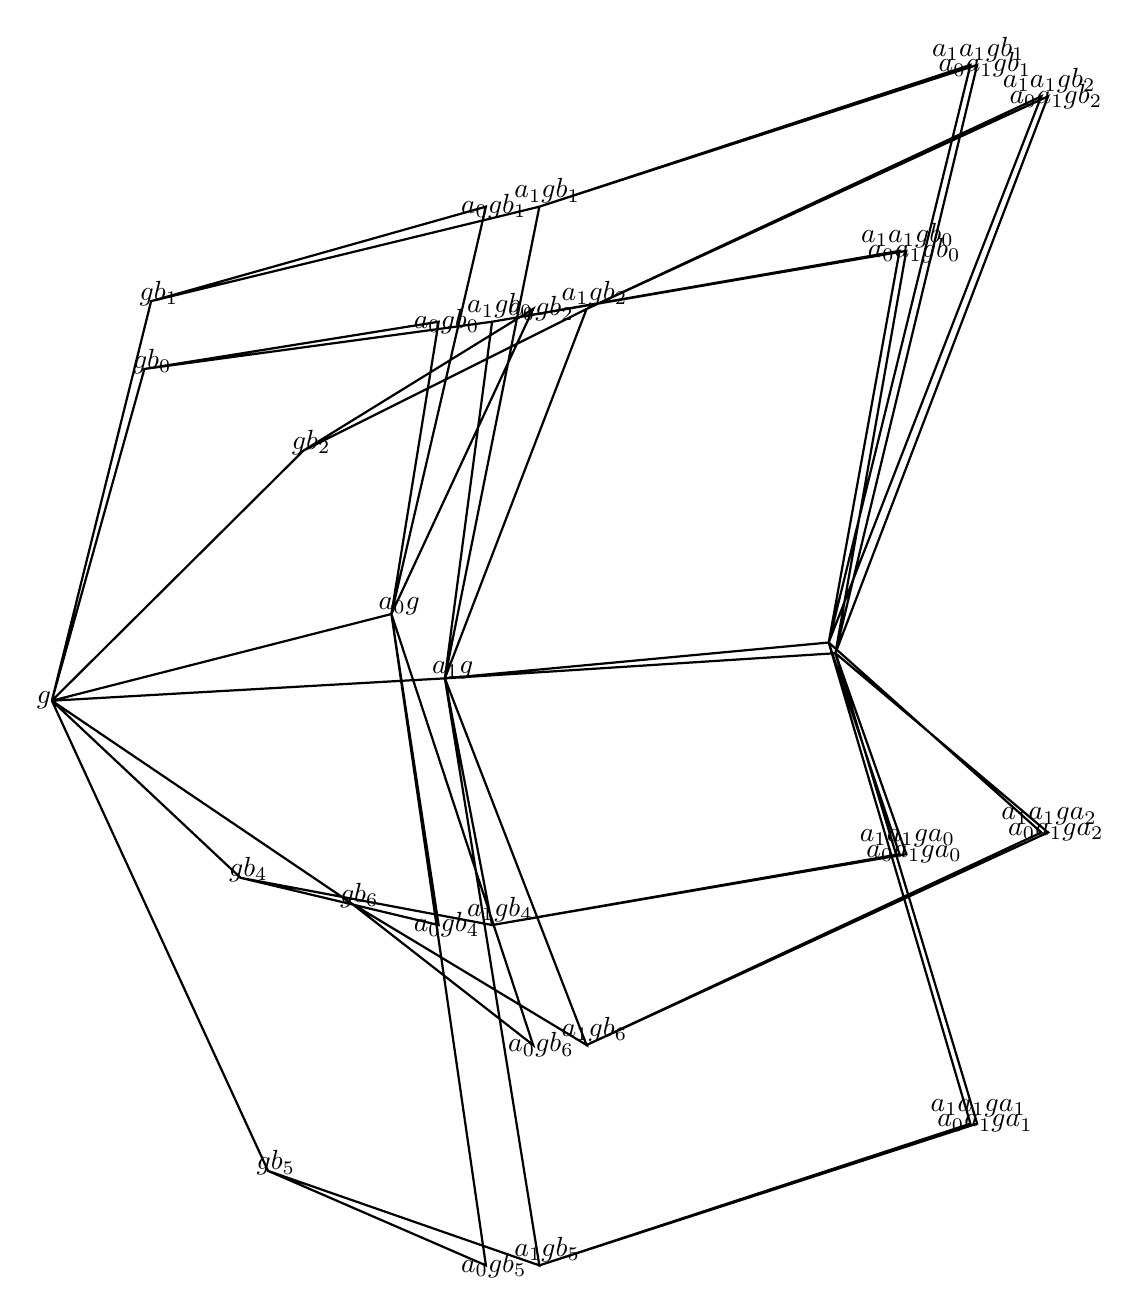
\begin{tikzpicture}
            \draw[thick](0,0)(0, 0) -- (1.1749577764927106,4.212986360061736) -- (4.912094726487489,4.8129863600617355) -- (4.312094726487489,1.1010251120238759) -- (0, 0)
(0, 0) -- (1.2604186852865784,5.07415775618791) -- (5.512094726487489,6.27415775618791) -- (4.312094726487489,1.1010251120238759) -- (0, 0)
(0, 0) -- (3.1937888577174833,3.1751509294849223) -- (6.112094726487489,4.975150929484922) -- (4.312094726487489,1.1010251120238759) -- (0, 0)
(0, 0) -- (1.1749577764927106,4.212986360061736) -- (5.590964870809898,4.8129863600617355) -- (4.990964870809898,0.2839101271553097) -- (0, 0)
(0, 0) -- (1.2604186852865784,5.07415775618791) -- (6.190964870809898,6.27415775618791) -- (4.990964870809898,0.2839101271553097) -- (0, 0)
(0, 0) -- (3.1937888577174833,3.1751509294849223) -- (6.790964870809898,4.975150929484922) -- (4.990964870809898,0.2839101271553097) -- (0, 0)
(0, 0) -- (2.3960928376757655,-2.2491431461566855) -- (4.912094726487489,-2.8491431461566856) -- (4.312094726487489,1.1010251120238759) -- (0, 0)
(0, 0) -- (2.745325214945222,-5.971308933567112) -- (5.512094726487489,-7.171308933567112) -- (4.312094726487489,1.1010251120238759) -- (0, 0)
(0, 0) -- (3.8042283149487215,-2.5730955918641296) -- (6.112094726487489,-4.373095591864129) -- (4.312094726487489,1.1010251120238759) -- (0, 0)
(0, 0) -- (2.3960928376757655,-2.2491431461566855) -- (5.590964870809898,-2.8491431461566856) -- (4.990964870809898,0.2839101271553097) -- (0, 0)
(0, 0) -- (2.745325214945222,-5.971308933567112) -- (6.190964870809898,-7.171308933567112) -- (4.990964870809898,0.2839101271553097) -- (0, 0)
(0, 0) -- (3.8042283149487215,-2.5730955918641296) -- (6.790964870809898,-4.373095591864129) -- (4.990964870809898,0.2839101271553097) -- (0, 0)
(4.990964870809898, 0.2839101271553097) -- (5.590964870809898,4.8129863600617355) -- (10.85099378292885,5.712986360061736) -- (9.95099378292885,0.6030658358612564) -- (4.990964870809898, 0.2839101271553097)
(4.990964870809898, 0.2839101271553097) -- (6.190964870809898,6.27415775618791) -- (11.75099378292885,8.07415775618791) -- (9.95099378292885,0.6030658358612564) -- (4.990964870809898, 0.2839101271553097)
(4.990964870809898, 0.2839101271553097) -- (6.790964870809898,4.975150929484922) -- (12.65099378292885,7.675150929484922) -- (9.95099378292885,0.6030658358612564) -- (4.990964870809898, 0.2839101271553097)
(4.990964870809898, 0.2839101271553097) -- (5.590964870809898,4.8129863600617355) -- (10.765579505543753,5.712986360061736) -- (9.865579505543753,0.739135293588209) -- (4.990964870809898, 0.2839101271553097)
(4.990964870809898, 0.2839101271553097) -- (6.190964870809898,6.27415775618791) -- (11.665579505543754,8.07415775618791) -- (9.865579505543753,0.739135293588209) -- (4.990964870809898, 0.2839101271553097)
(4.990964870809898, 0.2839101271553097) -- (6.790964870809898,4.975150929484922) -- (12.565579505543752,7.675150929484922) -- (9.865579505543753,0.739135293588209) -- (4.990964870809898, 0.2839101271553097)
(4.990964870809898, 0.2839101271553097) -- (5.590964870809898,-2.8491431461566856) -- (10.85099378292885,-1.9491431461566857) -- (9.95099378292885,0.6030658358612564) -- (4.990964870809898, 0.2839101271553097)
(4.990964870809898, 0.2839101271553097) -- (6.190964870809898,-7.171308933567112) -- (11.75099378292885,-5.3713089335671125) -- (9.95099378292885,0.6030658358612564) -- (4.990964870809898, 0.2839101271553097)
(4.990964870809898, 0.2839101271553097) -- (6.790964870809898,-4.373095591864129) -- (12.65099378292885,-1.6730955918641293) -- (9.95099378292885,0.6030658358612564) -- (4.990964870809898, 0.2839101271553097)
(4.990964870809898, 0.2839101271553097) -- (5.590964870809898,-2.8491431461566856) -- (10.765579505543753,-1.9491431461566857) -- (9.865579505543753,0.739135293588209) -- (4.990964870809898, 0.2839101271553097)
(4.990964870809898, 0.2839101271553097) -- (6.190964870809898,-7.171308933567112) -- (11.665579505543754,-5.3713089335671125) -- (9.865579505543753,0.739135293588209) -- (4.990964870809898, 0.2839101271553097)
(4.990964870809898, 0.2839101271553097) -- (6.790964870809898,-4.373095591864129) -- (12.565579505543752,-1.6730955918641293) -- (9.865579505543753,0.739135293588209) -- (4.990964870809898, 0.2839101271553097)
;
\node at (5.012094726487488,4.8129863600617355) {$ a_{ 0  } gb_{ 0 } $};
\node at (5.612094726487489,6.27415775618791) {$ a_{ 0  } gb_{ 1 } $};
\node at (6.212094726487488,4.975150929484922) {$ a_{ 0  } gb_{ 2 } $};
\node at (5.690964870809897,5.012986360061736) {$ a_{ 1  } gb_{ 0 } $};
\node at (6.290964870809898,6.4741577561879105) {$ a_{ 1  } gb_{ 1 } $};
\node at (6.890964870809897,5.175150929484922) {$ a_{ 1  } gb_{ 2 } $};
\node at (5.012094726487488,-2.8491431461566856) {$ a_{ 0  } gb_{ 4 } $};
\node at (5.612094726487489,-7.171308933567112) {$ a_{ 0  } gb_{ 5 } $};
\node at (6.212094726487488,-4.373095591864129) {$ a_{ 0  } gb_{ 6 } $};
\node at (5.690964870809897,-2.6491431461566854) {$ a_{ 1  } gb_{ 4 } $};
\node at (6.290964870809898,-6.971308933567112) {$ a_{ 1  } gb_{ 5 } $};
\node at (6.890964870809897,-4.173095591864129) {$ a_{ 1  } gb_{ 6 } $};
\node at (10.95099378292885,5.712986360061736) {$ a_{ 0  } a_{ 1 }gb_{ 0 } $};
\node at (11.85099378292885,8.07415775618791) {$ a_{ 0  } a_{ 1 }gb_{ 1 } $};
\node at (12.75099378292885,7.675150929484922) {$ a_{ 0  } a_{ 1 }gb_{ 2 } $};
\node at (10.865579505543753,5.912986360061736) {$ a_{ 1  } a_{ 1 }gb_{ 0 } $};
\node at (11.765579505543753,8.27415775618791) {$ a_{ 1  } a_{ 1 }gb_{ 1 } $};
\node at (12.665579505543752,7.8751509294849225) {$ a_{ 1  } a_{ 1 }gb_{ 2 } $};
\node at (10.95099378292885,-1.9491431461566857) {$ a_{ 0  } a_{ 1 }ga_{ 0 } $};
\node at (11.85099378292885,-5.3713089335671125) {$ a_{ 0  } a_{ 1 }ga_{ 1 } $};
\node at (12.75099378292885,-1.6730955918641293) {$ a_{ 0  } a_{ 1 }ga_{ 2 } $};
\node at (10.865579505543753,-1.7491431461566858) {$ a_{ 1  } a_{ 1 }ga_{ 0 } $};
\node at (11.765579505543753,-5.171308933567112) {$ a_{ 1  } a_{ 1 }ga_{ 1 } $};
\node at (12.665579505543752,-1.4730955918641293) {$ a_{ 1  } a_{ 1 }ga_{ 2 } $};
\node at (-0.1,0) {$ g $};
\node at (4.412094726487489,1.201025112023876) {$ a_{ 0 }g $};
\node at (5.090964870809898,0.3839101271553097) {$ a_{ 1 }g $};
\node at (1.2749577764927107,4.3129863600617355) {$ gb_{ 0 } $};
\node at (1.3604186852865785,5.17415775618791) {$ gb_{ 1 } $};
\node at (3.2937888577174834,3.2751509294849224) {$ gb_{ 2 } $};
\node at (2.4960928376757656,-2.1491431461566854) {$ gb_{ 4 } $};
\node at (2.845325214945222,-5.8713089335671125) {$ gb_{ 5 } $};
\node at (3.9042283149487216,-2.4730955918641295) {$ gb_{ 6 } $};

            \end{tikzpicture}
            \end{center}
            \caption{Square of the complex, with edges $(g,ag), (agb, gb) \in E_A,
            (g,gb), (agb, ag) \in E_B.$ \label{fig:square}
            }
            \end{figure}
 \begin{figure}[H]
            %\label{fig:square}
            \begin{center}
            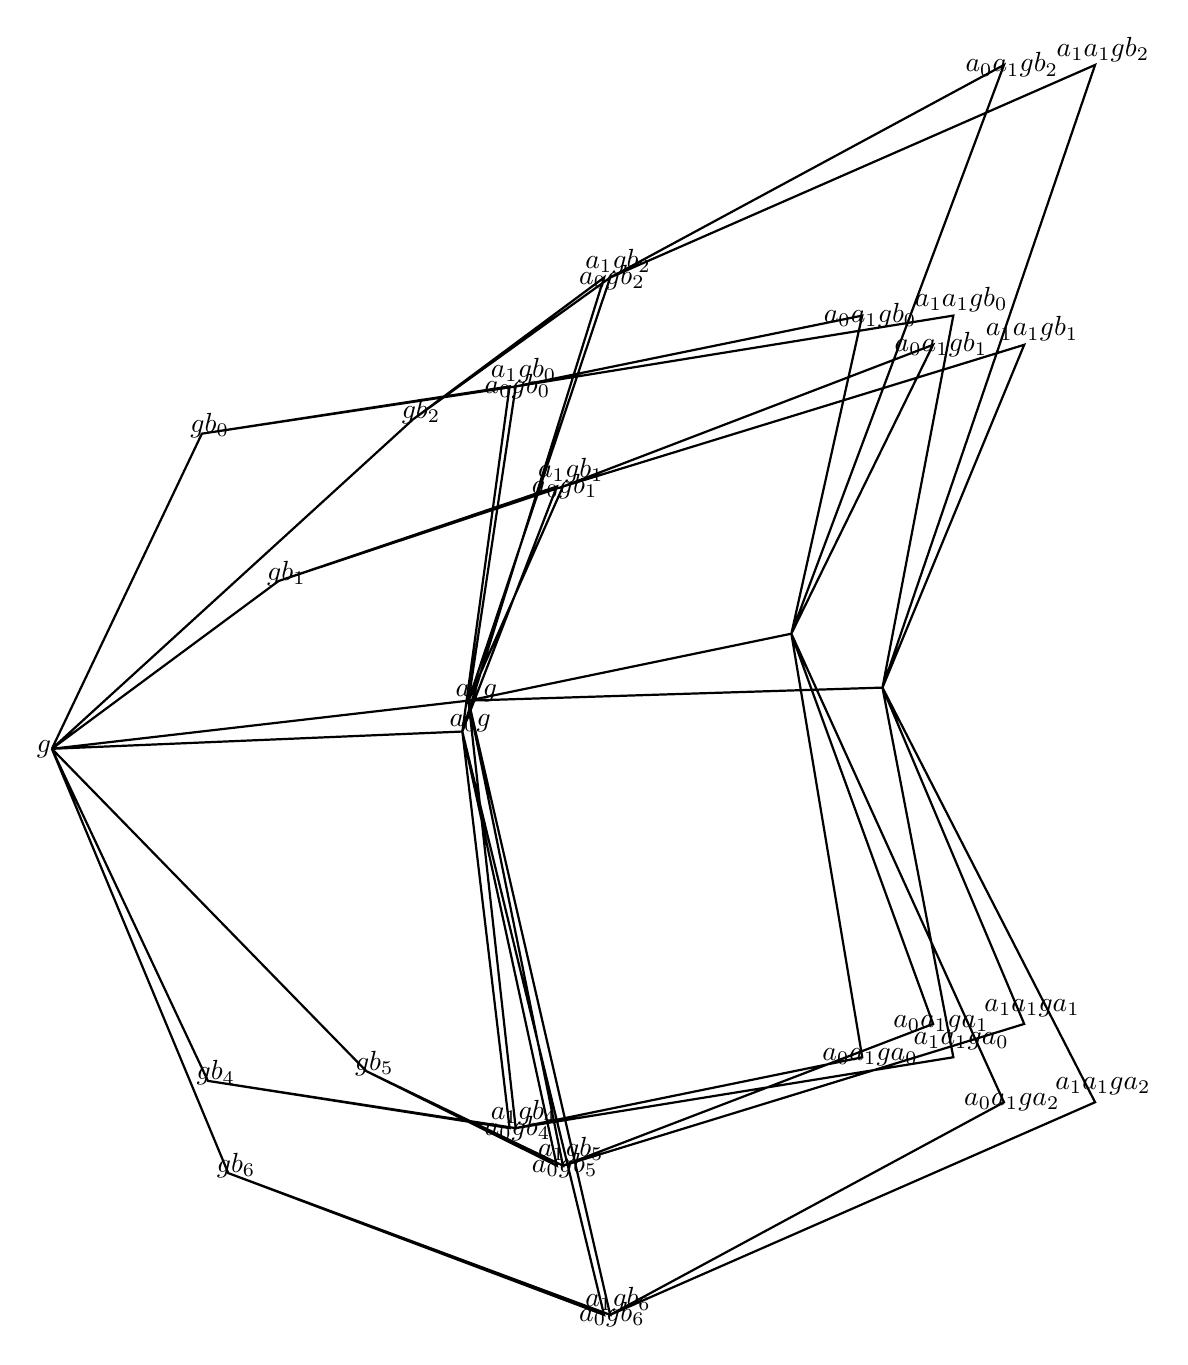
\begin{tikzpicture}
            \draw[thick](0,0)(0, 0) -- (1.9049911888377424,4.002079117547451) -- (5.81285084955138,4.602079117547451) -- (5.212850849551381,0.2192498173032679) -- (0, 0)
(0, 0) -- (2.879157898699928,2.130954290533681) -- (6.412850849551381,3.330954290533681) -- (5.212850849551381,0.2192498173032679) -- (0, 0)
(0, 0) -- (4.588270563356833,4.1850314105127575) -- (7.012850849551381,5.985031410512757) -- (5.212850849551381,0.2192498173032679) -- (0, 0)
(0, 0) -- (1.9049911888377424,4.002079117547451) -- (5.890590913653101,4.602079117547451) -- (5.2905909136531015,0.6119546131629411) -- (0, 0)
(0, 0) -- (2.879157898699928,2.130954290533681) -- (6.490590913653102,3.330954290533681) -- (5.2905909136531015,0.6119546131629411) -- (0, 0)
(0, 0) -- (4.588270563356833,4.1850314105127575) -- (7.090590913653101,5.985031410512757) -- (5.2905909136531015,0.6119546131629411) -- (0, 0)
(0, 0) -- (1.9818949186177792,-4.217396385887875) -- (5.81285084955138,-4.817396385887875) -- (5.212850849551381,0.2192498173032679) -- (0, 0)
(0, 0) -- (3.9944175473955323,-4.094159016671296) -- (6.412850849551381,-5.294159016671296) -- (5.212850849551381,0.2192498173032679) -- (0, 0)
(0, 0) -- (2.2401823432002748,-5.388664191428558) -- (7.012850849551381,-7.188664191428558) -- (5.212850849551381,0.2192498173032679) -- (0, 0)
(0, 0) -- (1.9818949186177792,-4.217396385887875) -- (5.890590913653101,-4.817396385887875) -- (5.2905909136531015,0.6119546131629411) -- (0, 0)
(0, 0) -- (3.9944175473955323,-4.094159016671296) -- (6.490590913653102,-5.294159016671296) -- (5.2905909136531015,0.6119546131629411) -- (0, 0)
(0, 0) -- (2.2401823432002748,-5.388664191428558) -- (7.090590913653101,-7.188664191428558) -- (5.2905909136531015,0.6119546131629411) -- (0, 0)
(5.2905909136531015, 0.6119546131629411) -- (5.890590913653101,4.602079117547451) -- (10.291575076901802,5.502079117547451) -- (9.391575076901802,1.4619219538089987) -- (5.2905909136531015, 0.6119546131629411)
(5.2905909136531015, 0.6119546131629411) -- (6.490590913653102,3.330954290533681) -- (11.191575076901803,5.130954290533681) -- (9.391575076901802,1.4619219538089987) -- (5.2905909136531015, 0.6119546131629411)
(5.2905909136531015, 0.6119546131629411) -- (7.090590913653101,5.985031410512757) -- (12.091575076901801,8.685031410512757) -- (9.391575076901802,1.4619219538089987) -- (5.2905909136531015, 0.6119546131629411)
(5.2905909136531015, 0.6119546131629411) -- (5.890590913653101,4.602079117547451) -- (11.4486392380322,5.502079117547451) -- (10.5486392380322,0.7771825477033486) -- (5.2905909136531015, 0.6119546131629411)
(5.2905909136531015, 0.6119546131629411) -- (6.490590913653102,3.330954290533681) -- (12.3486392380322,5.130954290533681) -- (10.5486392380322,0.7771825477033486) -- (5.2905909136531015, 0.6119546131629411)
(5.2905909136531015, 0.6119546131629411) -- (7.090590913653101,5.985031410512757) -- (13.248639238032201,8.685031410512757) -- (10.5486392380322,0.7771825477033486) -- (5.2905909136531015, 0.6119546131629411)
(5.2905909136531015, 0.6119546131629411) -- (5.890590913653101,-4.817396385887875) -- (10.291575076901802,-3.917396385887875) -- (9.391575076901802,1.4619219538089987) -- (5.2905909136531015, 0.6119546131629411)
(5.2905909136531015, 0.6119546131629411) -- (6.490590913653102,-5.294159016671296) -- (11.191575076901803,-3.494159016671296) -- (9.391575076901802,1.4619219538089987) -- (5.2905909136531015, 0.6119546131629411)
(5.2905909136531015, 0.6119546131629411) -- (7.090590913653101,-7.188664191428558) -- (12.091575076901801,-4.488664191428557) -- (9.391575076901802,1.4619219538089987) -- (5.2905909136531015, 0.6119546131629411)
(5.2905909136531015, 0.6119546131629411) -- (5.890590913653101,-4.817396385887875) -- (11.4486392380322,-3.917396385887875) -- (10.5486392380322,0.7771825477033486) -- (5.2905909136531015, 0.6119546131629411)
(5.2905909136531015, 0.6119546131629411) -- (6.490590913653102,-5.294159016671296) -- (12.3486392380322,-3.494159016671296) -- (10.5486392380322,0.7771825477033486) -- (5.2905909136531015, 0.6119546131629411)
(5.2905909136531015, 0.6119546131629411) -- (7.090590913653101,-7.188664191428558) -- (13.248639238032201,-4.488664191428557) -- (10.5486392380322,0.7771825477033486) -- (5.2905909136531015, 0.6119546131629411)
;
\node at (5.91285084955138,4.602079117547451) {$ a_{ 0  } gb_{ 0 } $};
\node at (6.512850849551381,3.330954290533681) {$ a_{ 0  } gb_{ 1 } $};
\node at (7.11285084955138,5.985031410512757) {$ a_{ 0  } gb_{ 2 } $};
\node at (5.990590913653101,4.802079117547451) {$ a_{ 1  } gb_{ 0 } $};
\node at (6.590590913653101,3.530954290533681) {$ a_{ 1  } gb_{ 1 } $};
\node at (7.190590913653101,6.1850314105127575) {$ a_{ 1  } gb_{ 2 } $};
\node at (5.91285084955138,-4.817396385887875) {$ a_{ 0  } gb_{ 4 } $};
\node at (6.512850849551381,-5.294159016671296) {$ a_{ 0  } gb_{ 5 } $};
\node at (7.11285084955138,-7.188664191428558) {$ a_{ 0  } gb_{ 6 } $};
\node at (5.990590913653101,-4.617396385887875) {$ a_{ 1  } gb_{ 4 } $};
\node at (6.590590913653101,-5.094159016671296) {$ a_{ 1  } gb_{ 5 } $};
\node at (7.190590913653101,-6.988664191428557) {$ a_{ 1  } gb_{ 6 } $};
\node at (10.391575076901802,5.502079117547451) {$ a_{ 0  } a_{ 1 }gb_{ 0 } $};
\node at (11.291575076901802,5.130954290533681) {$ a_{ 0  } a_{ 1 }gb_{ 1 } $};
\node at (12.1915750769018,8.685031410512757) {$ a_{ 0  } a_{ 1 }gb_{ 2 } $};
\node at (11.5486392380322,5.702079117547451) {$ a_{ 1  } a_{ 1 }gb_{ 0 } $};
\node at (12.4486392380322,5.330954290533681) {$ a_{ 1  } a_{ 1 }gb_{ 1 } $};
\node at (13.3486392380322,8.885031410512756) {$ a_{ 1  } a_{ 1 }gb_{ 2 } $};
\node at (10.391575076901802,-3.917396385887875) {$ a_{ 0  } a_{ 1 }ga_{ 0 } $};
\node at (11.291575076901802,-3.494159016671296) {$ a_{ 0  } a_{ 1 }ga_{ 1 } $};
\node at (12.1915750769018,-4.488664191428557) {$ a_{ 0  } a_{ 1 }ga_{ 2 } $};
\node at (11.5486392380322,-3.717396385887875) {$ a_{ 1  } a_{ 1 }ga_{ 0 } $};
\node at (12.4486392380322,-3.294159016671296) {$ a_{ 1  } a_{ 1 }ga_{ 1 } $};
\node at (13.3486392380322,-4.288664191428557) {$ a_{ 1  } a_{ 1 }ga_{ 2 } $};
\node at (-0.1,0) {$ g $};
\node at (5.31285084955138,0.3192498173032679) {$ a_{ 0 }g $};
\node at (5.390590913653101,0.7119546131629411) {$ a_{ 1 }g $};
\node at (2.0049911888377423,4.102079117547451) {$ gb_{ 0 } $};
\node at (2.979157898699928,2.230954290533681) {$ gb_{ 1 } $};
\node at (4.6882705633568325,4.285031410512757) {$ gb_{ 2 } $};
\node at (2.0818949186177793,-4.117396385887876) {$ gb_{ 4 } $};
\node at (4.094417547395532,-3.9941590166712957) {$ gb_{ 5 } $};
\node at (2.340182343200275,-5.288664191428558) {$ gb_{ 6 } $};

            \end{tikzpicture}
            \end{center}
            \caption{Square of the complex, with edges $(g,ag), (agb, gb) \in E_A,
            (g,gb), (agb, ag) \in E_B.$ \label{fig:square}
            }
            \end{figure}
 \begin{figure}[H]
            %\label{fig:square}
            \begin{center}
            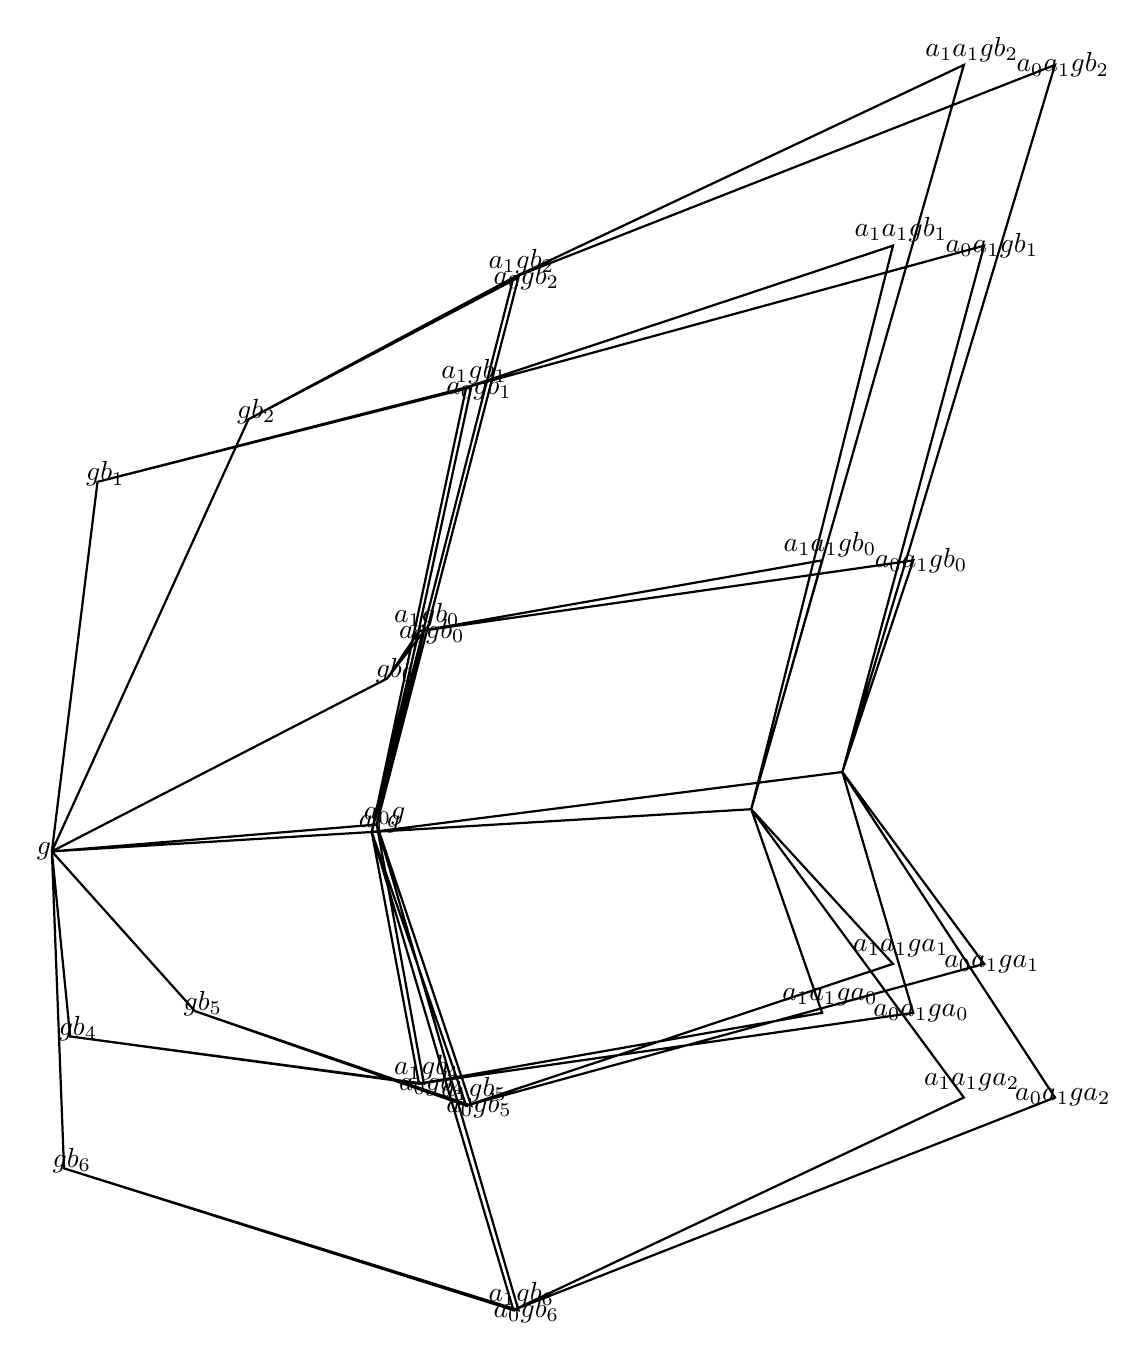
\begin{tikzpicture}
            \draw[thick](0,0)(0, 0) -- (4.2581060002527105,2.1962957942483303) -- (4.72555547758494,2.7962957942483304) -- (4.125555477584941,0.34146397975939063) -- (0, 0)
(0, 0) -- (0.5798318376318434,4.6932423622867265) -- (5.325555477584941,5.893242362286727) -- (4.125555477584941,0.34146397975939063) -- (0, 0)
(0, 0) -- (2.496712870407998,5.488028826701058) -- (5.925555477584941,7.288028826701058) -- (4.125555477584941,0.34146397975939063) -- (0, 0)
(0, 0) -- (4.2581060002527105,2.1962957942483303) -- (4.662084276222307,2.7962957942483304) -- (4.062084276222308,0.24654513566212666) -- (0, 0)
(0, 0) -- (0.5798318376318434,4.6932423622867265) -- (5.262084276222308,5.893242362286727) -- (4.062084276222308,0.24654513566212666) -- (0, 0)
(0, 0) -- (2.496712870407998,5.488028826701058) -- (5.8620842762223075,7.288028826701058) -- (4.062084276222308,0.24654513566212666) -- (0, 0)
(0, 0) -- (0.2323381597493146,-2.3499782654285317) -- (4.72555547758494,-2.949978265428532) -- (4.125555477584941,0.34146397975939063) -- (0, 0)
(0, 0) -- (1.8175377296441309,-2.028344076200503) -- (5.325555477584941,-3.2283440762005027) -- (4.125555477584941,0.34146397975939063) -- (0, 0)
(0, 0) -- (0.15448807084038618,-4.025534995011849) -- (5.925555477584941,-5.825534995011849) -- (4.125555477584941,0.34146397975939063) -- (0, 0)
(0, 0) -- (0.2323381597493146,-2.3499782654285317) -- (4.662084276222307,-2.949978265428532) -- (4.062084276222308,0.24654513566212666) -- (0, 0)
(0, 0) -- (1.8175377296441309,-2.028344076200503) -- (5.262084276222308,-3.2283440762005027) -- (4.062084276222308,0.24654513566212666) -- (0, 0)
(0, 0) -- (0.15448807084038618,-4.025534995011849) -- (5.8620842762223075,-5.825534995011849) -- (4.062084276222308,0.24654513566212666) -- (0, 0)
(4.062084276222308, 0.24654513566212666) -- (4.662084276222307,2.7962957942483304) -- (10.93933403194493,3.6962957942483303) -- (10.03933403194493,1.0083246395114376) -- (4.062084276222308, 0.24654513566212666)
(4.062084276222308, 0.24654513566212666) -- (5.262084276222308,5.893242362286727) -- (11.839334031944931,7.6932423622867265) -- (10.03933403194493,1.0083246395114376) -- (4.062084276222308, 0.24654513566212666)
(4.062084276222308, 0.24654513566212666) -- (5.8620842762223075,7.288028826701058) -- (12.739334031944932,9.988028826701058) -- (10.03933403194493,1.0083246395114376) -- (4.062084276222308, 0.24654513566212666)
(4.062084276222308, 0.24654513566212666) -- (4.662084276222307,2.7962957942483304) -- (9.781904738187622,3.6962957942483303) -- (8.881904738187622,0.5358514939262355) -- (4.062084276222308, 0.24654513566212666)
(4.062084276222308, 0.24654513566212666) -- (5.262084276222308,5.893242362286727) -- (10.681904738187622,7.6932423622867265) -- (8.881904738187622,0.5358514939262355) -- (4.062084276222308, 0.24654513566212666)
(4.062084276222308, 0.24654513566212666) -- (5.8620842762223075,7.288028826701058) -- (11.581904738187621,9.988028826701058) -- (8.881904738187622,0.5358514939262355) -- (4.062084276222308, 0.24654513566212666)
(4.062084276222308, 0.24654513566212666) -- (4.662084276222307,-2.949978265428532) -- (10.93933403194493,-2.049978265428532) -- (10.03933403194493,1.0083246395114376) -- (4.062084276222308, 0.24654513566212666)
(4.062084276222308, 0.24654513566212666) -- (5.262084276222308,-3.2283440762005027) -- (11.839334031944931,-1.4283440762005026) -- (10.03933403194493,1.0083246395114376) -- (4.062084276222308, 0.24654513566212666)
(4.062084276222308, 0.24654513566212666) -- (5.8620842762223075,-5.825534995011849) -- (12.739334031944932,-3.125534995011849) -- (10.03933403194493,1.0083246395114376) -- (4.062084276222308, 0.24654513566212666)
(4.062084276222308, 0.24654513566212666) -- (4.662084276222307,-2.949978265428532) -- (9.781904738187622,-2.049978265428532) -- (8.881904738187622,0.5358514939262355) -- (4.062084276222308, 0.24654513566212666)
(4.062084276222308, 0.24654513566212666) -- (5.262084276222308,-3.2283440762005027) -- (10.681904738187622,-1.4283440762005026) -- (8.881904738187622,0.5358514939262355) -- (4.062084276222308, 0.24654513566212666)
(4.062084276222308, 0.24654513566212666) -- (5.8620842762223075,-5.825534995011849) -- (11.581904738187621,-3.125534995011849) -- (8.881904738187622,0.5358514939262355) -- (4.062084276222308, 0.24654513566212666)
;
\node at (4.82555547758494,2.7962957942483304) {$ a_{ 0  } gb_{ 0 } $};
\node at (5.425555477584941,5.893242362286727) {$ a_{ 0  } gb_{ 1 } $};
\node at (6.02555547758494,7.288028826701058) {$ a_{ 0  } gb_{ 2 } $};
\node at (4.762084276222307,2.9962957942483306) {$ a_{ 1  } gb_{ 0 } $};
\node at (5.3620842762223075,6.093242362286727) {$ a_{ 1  } gb_{ 1 } $};
\node at (5.962084276222307,7.488028826701058) {$ a_{ 1  } gb_{ 2 } $};
\node at (4.82555547758494,-2.949978265428532) {$ a_{ 0  } gb_{ 4 } $};
\node at (5.425555477584941,-3.2283440762005027) {$ a_{ 0  } gb_{ 5 } $};
\node at (6.02555547758494,-5.825534995011849) {$ a_{ 0  } gb_{ 6 } $};
\node at (4.762084276222307,-2.7499782654285316) {$ a_{ 1  } gb_{ 4 } $};
\node at (5.3620842762223075,-3.0283440762005025) {$ a_{ 1  } gb_{ 5 } $};
\node at (5.962084276222307,-5.625534995011849) {$ a_{ 1  } gb_{ 6 } $};
\node at (11.03933403194493,3.6962957942483303) {$ a_{ 0  } a_{ 1 }gb_{ 0 } $};
\node at (11.93933403194493,7.6932423622867265) {$ a_{ 0  } a_{ 1 }gb_{ 1 } $};
\node at (12.839334031944931,9.988028826701058) {$ a_{ 0  } a_{ 1 }gb_{ 2 } $};
\node at (9.881904738187622,3.8962957942483305) {$ a_{ 1  } a_{ 1 }gb_{ 0 } $};
\node at (10.781904738187622,7.893242362286727) {$ a_{ 1  } a_{ 1 }gb_{ 1 } $};
\node at (11.68190473818762,10.188028826701057) {$ a_{ 1  } a_{ 1 }gb_{ 2 } $};
\node at (11.03933403194493,-2.049978265428532) {$ a_{ 0  } a_{ 1 }ga_{ 0 } $};
\node at (11.93933403194493,-1.4283440762005026) {$ a_{ 0  } a_{ 1 }ga_{ 1 } $};
\node at (12.839334031944931,-3.125534995011849) {$ a_{ 0  } a_{ 1 }ga_{ 2 } $};
\node at (9.881904738187622,-1.849978265428532) {$ a_{ 1  } a_{ 1 }ga_{ 0 } $};
\node at (10.781904738187622,-1.2283440762005027) {$ a_{ 1  } a_{ 1 }ga_{ 1 } $};
\node at (11.68190473818762,-2.9255349950118488) {$ a_{ 1  } a_{ 1 }ga_{ 2 } $};
\node at (-0.1,0) {$ g $};
\node at (4.22555547758494,0.44146397975939067) {$ a_{ 0 }g $};
\node at (4.162084276222307,0.34654513566212664) {$ a_{ 1 }g $};
\node at (4.35810600025271,2.2962957942483304) {$ gb_{ 0 } $};
\node at (0.6798318376318434,4.793242362286726) {$ gb_{ 1 } $};
\node at (2.5967128704079983,5.588028826701057) {$ gb_{ 2 } $};
\node at (0.3323381597493146,-2.2499782654285316) {$ gb_{ 4 } $};
\node at (1.917537729644131,-1.9283440762005029) {$ gb_{ 5 } $};
\node at (0.25448807084038616,-3.925534995011849) {$ gb_{ 6 } $};

            \end{tikzpicture}
            \end{center}
            \caption{Square of the complex, with edges $(g,ag), (agb, gb) \in E_A,
            (g,gb), (agb, ag) \in E_B.$ \label{fig:square}
            }
            \end{figure}
 \begin{figure}[H]
            %\label{fig:square}
            \begin{center}
            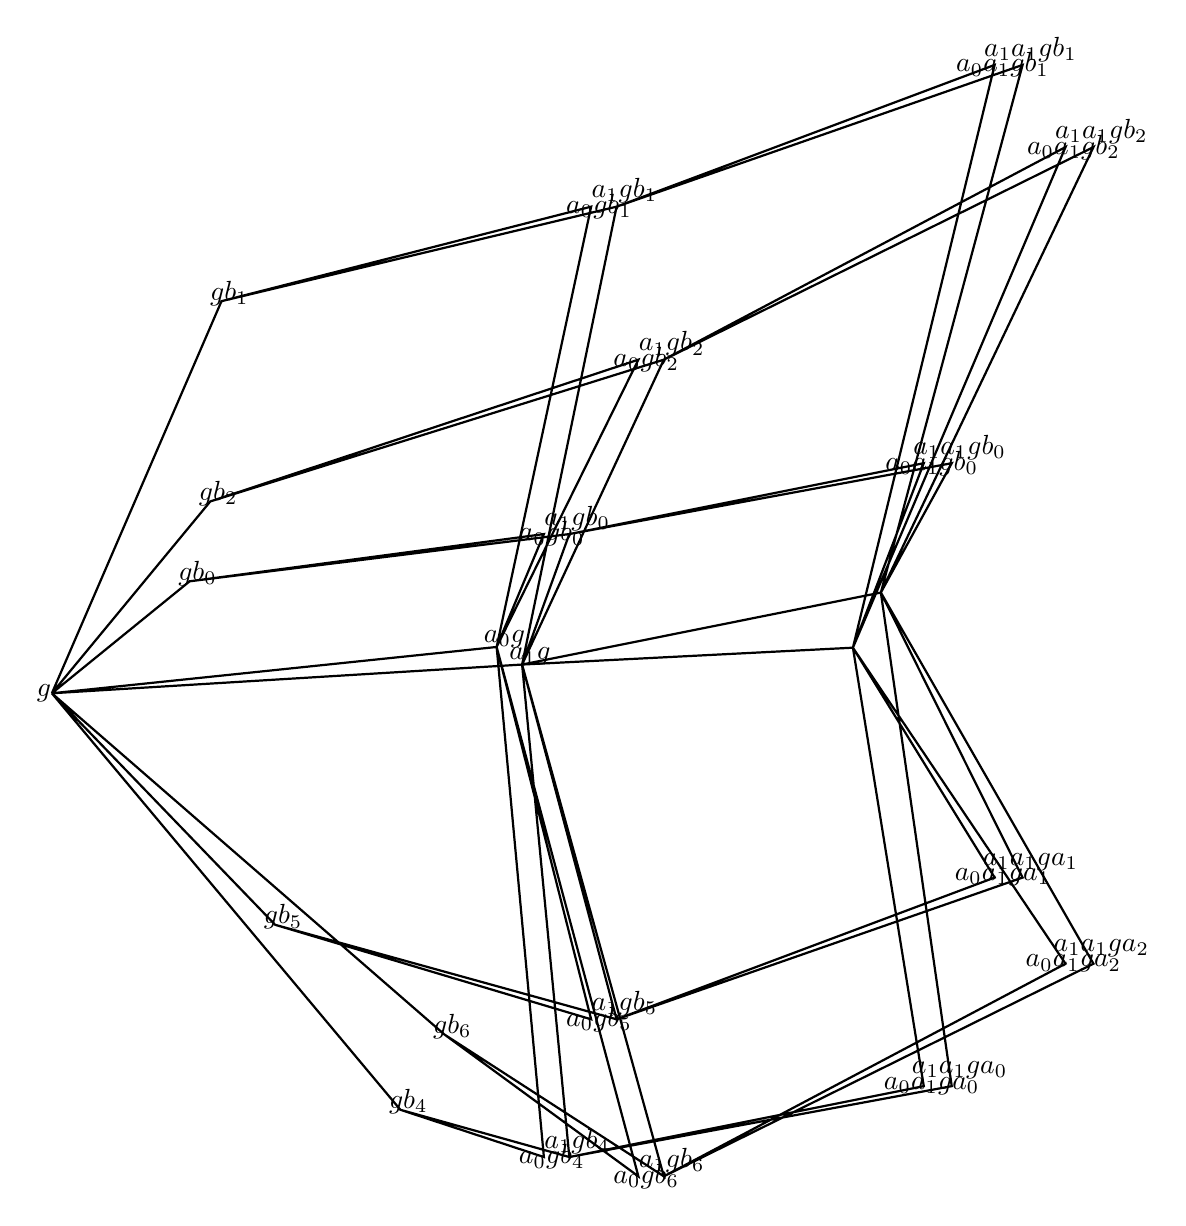
\begin{tikzpicture}
            \draw[thick](0,0)(0, 0) -- (1.7495997892644493,1.4219726253058653) -- (6.248599546296113,2.021972625305865) -- (5.648599546296113,0.5880300813598297) -- (0, 0)
(0, 0) -- (2.1545355270094517,4.979884294074534) -- (6.848599546296113,6.179884294074534) -- (5.648599546296113,0.5880300813598297) -- (0, 0)
(0, 0) -- (2.012358237892944,2.4366833147068805) -- (7.448599546296113,4.23668331470688) -- (5.648599546296113,0.5880300813598297) -- (0, 0)
(0, 0) -- (1.7495997892644493,1.4219726253058653) -- (6.571813815137887,2.021972625305865) -- (5.971813815137887,0.364845734892881) -- (0, 0)
(0, 0) -- (2.1545355270094517,4.979884294074534) -- (7.171813815137887,6.179884294074534) -- (5.971813815137887,0.364845734892881) -- (0, 0)
(0, 0) -- (2.012358237892944,2.4366833147068805) -- (7.771813815137887,4.23668331470688) -- (5.971813815137887,0.364845734892881) -- (0, 0)
(0, 0) -- (4.426068300908224,-5.28951942746695) -- (6.248599546296113,-5.88951942746695) -- (5.648599546296113,0.5880300813598297) -- (0, 0)
(0, 0) -- (2.8362413494662198,-2.940431402940203) -- (6.848599546296113,-4.140431402940203) -- (5.648599546296113,0.5880300813598297) -- (0, 0)
(0, 0) -- (4.986745116425172,-4.334476832255016) -- (7.448599546296113,-6.134476832255015) -- (5.648599546296113,0.5880300813598297) -- (0, 0)
(0, 0) -- (4.426068300908224,-5.28951942746695) -- (6.571813815137887,-5.88951942746695) -- (5.971813815137887,0.364845734892881) -- (0, 0)
(0, 0) -- (2.8362413494662198,-2.940431402940203) -- (7.171813815137887,-4.140431402940203) -- (5.971813815137887,0.364845734892881) -- (0, 0)
(0, 0) -- (4.986745116425172,-4.334476832255016) -- (7.771813815137887,-6.134476832255015) -- (5.971813815137887,0.364845734892881) -- (0, 0)
(5.971813815137887, 0.364845734892881) -- (6.571813815137887,2.021972625305865) -- (11.073209897401364,2.921972625305865) -- (10.173209897401364,0.578993287175482) -- (5.971813815137887, 0.364845734892881)
(5.971813815137887, 0.364845734892881) -- (7.171813815137887,6.179884294074534) -- (11.973209897401365,7.979884294074534) -- (10.173209897401364,0.578993287175482) -- (5.971813815137887, 0.364845734892881)
(5.971813815137887, 0.364845734892881) -- (7.771813815137887,4.23668331470688) -- (12.873209897401363,6.9366833147068805) -- (10.173209897401364,0.578993287175482) -- (5.971813815137887, 0.364845734892881)
(5.971813815137887, 0.364845734892881) -- (6.571813815137887,2.021972625305865) -- (11.428133433304872,2.921972625305865) -- (10.528133433304872,1.2791258394161864) -- (5.971813815137887, 0.364845734892881)
(5.971813815137887, 0.364845734892881) -- (7.171813815137887,6.179884294074534) -- (12.328133433304872,7.979884294074534) -- (10.528133433304872,1.2791258394161864) -- (5.971813815137887, 0.364845734892881)
(5.971813815137887, 0.364845734892881) -- (7.771813815137887,4.23668331470688) -- (13.228133433304873,6.9366833147068805) -- (10.528133433304872,1.2791258394161864) -- (5.971813815137887, 0.364845734892881)
(5.971813815137887, 0.364845734892881) -- (6.571813815137887,-5.88951942746695) -- (11.073209897401364,-4.989519427466949) -- (10.173209897401364,0.578993287175482) -- (5.971813815137887, 0.364845734892881)
(5.971813815137887, 0.364845734892881) -- (7.171813815137887,-4.140431402940203) -- (11.973209897401365,-2.3404314029402036) -- (10.173209897401364,0.578993287175482) -- (5.971813815137887, 0.364845734892881)
(5.971813815137887, 0.364845734892881) -- (7.771813815137887,-6.134476832255015) -- (12.873209897401363,-3.434476832255015) -- (10.173209897401364,0.578993287175482) -- (5.971813815137887, 0.364845734892881)
(5.971813815137887, 0.364845734892881) -- (6.571813815137887,-5.88951942746695) -- (11.428133433304872,-4.989519427466949) -- (10.528133433304872,1.2791258394161864) -- (5.971813815137887, 0.364845734892881)
(5.971813815137887, 0.364845734892881) -- (7.171813815137887,-4.140431402940203) -- (12.328133433304872,-2.3404314029402036) -- (10.528133433304872,1.2791258394161864) -- (5.971813815137887, 0.364845734892881)
(5.971813815137887, 0.364845734892881) -- (7.771813815137887,-6.134476832255015) -- (13.228133433304873,-3.434476832255015) -- (10.528133433304872,1.2791258394161864) -- (5.971813815137887, 0.364845734892881)
;
\node at (6.3485995462961125,2.021972625305865) {$ a_{ 0  } gb_{ 0 } $};
\node at (6.948599546296113,6.179884294074534) {$ a_{ 0  } gb_{ 1 } $};
\node at (7.548599546296113,4.23668331470688) {$ a_{ 0  } gb_{ 2 } $};
\node at (6.671813815137886,2.2219726253058654) {$ a_{ 1  } gb_{ 0 } $};
\node at (7.271813815137887,6.379884294074534) {$ a_{ 1  } gb_{ 1 } $};
\node at (7.8718138151378865,4.4366833147068805) {$ a_{ 1  } gb_{ 2 } $};
\node at (6.3485995462961125,-5.88951942746695) {$ a_{ 0  } gb_{ 4 } $};
\node at (6.948599546296113,-4.140431402940203) {$ a_{ 0  } gb_{ 5 } $};
\node at (7.548599546296113,-6.134476832255015) {$ a_{ 0  } gb_{ 6 } $};
\node at (6.671813815137886,-5.68951942746695) {$ a_{ 1  } gb_{ 4 } $};
\node at (7.271813815137887,-3.940431402940203) {$ a_{ 1  } gb_{ 5 } $};
\node at (7.8718138151378865,-5.934476832255015) {$ a_{ 1  } gb_{ 6 } $};
\node at (11.173209897401364,2.921972625305865) {$ a_{ 0  } a_{ 1 }gb_{ 0 } $};
\node at (12.073209897401364,7.979884294074534) {$ a_{ 0  } a_{ 1 }gb_{ 1 } $};
\node at (12.973209897401363,6.9366833147068805) {$ a_{ 0  } a_{ 1 }gb_{ 2 } $};
\node at (11.528133433304872,3.1219726253058653) {$ a_{ 1  } a_{ 1 }gb_{ 0 } $};
\node at (12.428133433304872,8.179884294074533) {$ a_{ 1  } a_{ 1 }gb_{ 1 } $};
\node at (13.328133433304872,7.136683314706881) {$ a_{ 1  } a_{ 1 }gb_{ 2 } $};
\node at (11.173209897401364,-4.989519427466949) {$ a_{ 0  } a_{ 1 }ga_{ 0 } $};
\node at (12.073209897401364,-2.3404314029402036) {$ a_{ 0  } a_{ 1 }ga_{ 1 } $};
\node at (12.973209897401363,-3.434476832255015) {$ a_{ 0  } a_{ 1 }ga_{ 2 } $};
\node at (11.528133433304872,-4.789519427466949) {$ a_{ 1  } a_{ 1 }ga_{ 0 } $};
\node at (12.428133433304872,-2.1404314029402034) {$ a_{ 1  } a_{ 1 }ga_{ 1 } $};
\node at (13.328133433304872,-3.234476832255015) {$ a_{ 1  } a_{ 1 }ga_{ 2 } $};
\node at (-0.1,0) {$ g $};
\node at (5.748599546296113,0.6880300813598297) {$ a_{ 0 }g $};
\node at (6.071813815137887,0.46484573489288106) {$ a_{ 1 }g $};
\node at (1.8495997892644493,1.5219726253058654) {$ gb_{ 0 } $};
\node at (2.254535527009452,5.0798842940745335) {$ gb_{ 1 } $};
\node at (2.112358237892944,2.5366833147068806) {$ gb_{ 2 } $};
\node at (4.526068300908223,-5.1895194274669505) {$ gb_{ 4 } $};
\node at (2.93624134946622,-2.840431402940203) {$ gb_{ 5 } $};
\node at (5.086745116425171,-4.234476832255016) {$ gb_{ 6 } $};

            \end{tikzpicture}
            \end{center}
            \caption{Square of the complex, with edges $(g,ag), (agb, gb) \in E_A,
            (g,gb), (agb, ag) \in E_B.$ \label{fig:square}
            }
            \end{figure}
 
%\end{multicols*}
  % \printbibliography 
\end{document}

 